\chapter*{Dodatak: Prikaz aktivnosti grupe}
		\addcontentsline{toc}{chapter}{Dodatak: Prikaz aktivnosti grupe}
		
		\section*{Dnevnik sastajanja}
		
		%\textbf{\textit{Kontinuirano osvježavanje}}\\
		
		\begin{packed_enum}
			\item  sastanak
			
			\item[] \begin{packed_item}
				\item Datum: 14. listopada 2022
				\item Prisustvovali: D.Kiramarios, D.Kovačević, K.Tomičić, D.Jambrović, K.Orešković, K.Kijac, S.Barac
				\item Teme sastanka:
				\begin{packed_item}
					\item  raspodjela uloga (podjela poslova na frontend, backend i razvoj dokumentacije)
					\item  rasprava o zadanoj temi
					\item  sakupljanje pitanja za prvi sastanak sa asistenticom
				\end{packed_item}
			\end{packed_item}
			
			\item  sastanak
			\item[] \begin{packed_item}
				\item Datum: 20. listopada 2022
				\item Prisustvovali: D.Kiramarios, D.Kovačević, K.Tomičić, D.Jambrović, K.Orešković, K.Kijac, S.Barac
				\item Teme sastanka:
				\begin{packed_item}
					\item  osnovni podaci o izvođenju projekta
					\item  postavljanje pitanja vezanih za implementaciju projekta asistentici tijekom prvih pola sata sastanka i sljedećih 20 min
				\end{packed_item}
			\end{packed_item}

			\item  sastanak
			\item[] \begin{packed_item}
				\item Datum: 20. listopada 2022
				\item Prisustvovali: D.Kiramarios, D.Kovačević, K.Tomičić, D.Jambrović, K.Orešković, K.Kijac, S.Barac
				\item Teme sastanka:
				\begin{packed_item}
					\item  detaljna analiza zadatka
					\item  planiranje raspodjele poslova tijekom sljedećeg tjedna vezanih za inicijalizaciju backenda, frontenda i dokumentacije
					\item  dogovor o korištenju Jire za bolje praćenje raspodjele poslova
				\end{packed_item}
			\end{packed_item}

			\eject

			\item  sastanak
			\item[] \begin{packed_item}
				\item Datum: 23. listopada 2022
				\item Prisustvovali: D.Kiramarios, D.Kovačević, K.Tomičić, D.Jambrović, K.Orešković, K.Kijac, S.Barac
				\item Teme sastanka:
				\begin{packed_item}
					\item  pregled predložene skice klijentske aplikacije (frontend)
					\item  pregled predložene sheme za bazu podataka (backend)
					\item  pregled obrazaca uporabe i UC dijagrama (dokumentacija)
					\item  zaključak: male promjene sheme baze i slanje na pregled asistentici
				\end{packed_item}
			\end{packed_item}

			\item  sastanak
			\item[] \begin{packed_item}
				\item Datum: 24. listopada 2022
				\item Prisustvovali: D.Kiramarios, K.Tomičić, S.Barac
				\item Teme sastanka:
				\begin{packed_item}
					\item  detaljna analiza prijedloga dizajna za klijentsku aplikaciju
					\item  male promjene dizajna za klijentsku aplikaciju
					\item  podjela posla na klijentskoj aplikaciji među prisutnima
				\end{packed_item}
			\end{packed_item}

			\item  sastanak
			\item[] \begin{packed_item}
				\item Datum: 31. listopada 2022
				\item Prisustvovali: D.Kiramarios, K.Tomičić, S.Barac
				\item Teme sastanka:
				\begin{packed_item}
					\item  podjela posla na izradu routinga, izgleda, određenih komponenti i spajanja s backendom
				\end{packed_item}
			\end{packed_item}

			\item  sastanak
			\item[] \begin{packed_item}
				\item Datum: 3. studenoga 2022
				\item Prisustvovali: D.Kiramarios, D.Kovačević, K.Tomičić, D.Jambrović, K.Orešković, K.Kijac, S.Barac
				\item Teme sastanka:
				\begin{packed_item}
					\item pregled napravljene dokumentacije s asistenticom
					\item savjeti oko potrebnih promjena dokumentacije
					\item razgovor o implementaciji konkretnih svari na frontendu i backendu
				\end{packed_item}
			\end{packed_item}

			\eject

			\item  sastanak
			\item[] \begin{packed_item}
				\item Datum: 5. studenoga 2022
				\item Prisustvovali: K.Kijac, D.Jambrović
				\item Teme sastanka:
				\begin{packed_item}
					\item pregled prve verzije dokumentacije
					\item podjela posla oko finalnih promjena prve verzije dokumentacije
				\end{packed_item}
			\end{packed_item}

			\item  sastanak
			\item[] \begin{packed_item}
				\item Datum: 8. studenoga 2022
				\item Prisustvovali: D.Kiramarios, D.Kovačević, K.Orešković, S.Barac
				\item Teme sastanka:
				\begin{packed_item}
					\item spajanje frontenda i backenda (integracija API poziva)
				\end{packed_item}
			\end{packed_item}

			\item  sastanak
			\item[] \begin{packed_item}
				\item Datum: 9. studenoga 2022
				\item Prisustvovali: D.Kiramarios, K.Tomičić, S.Barac
				\item Teme sastanka:
				\begin{packed_item}
					\item daljnji planovi oko podjele posla na frontendu
					\item priprema za deploy prve inačice
				\end{packed_item}
			\end{packed_item}

			\item  sastanak
			\item[] \begin{packed_item}
				\item Datum: 10. studenoga 2022
				\item Prisustvovali: K.Orešković, D.Jambrović
				\item Teme sastanka:
				\begin{packed_item}
					\item pregled i diskusija dijagrama razreda
				\end{packed_item}
			\end{packed_item}

			\item  sastanak
			\item[] \begin{packed_item}
				\item Datum: 10. studenoga 2022
				\item Prisustvovali: D.Kiramarios, K. Kijac
				\item Teme sastanka:
				\begin{packed_item}
					\item provjera sekvencijskih dijagrama
				\end{packed_item}
			\end{packed_item}

			\item  sastanak
			\item[] \begin{packed_item}
				\item Datum: 5. prosinca 2022
				\item Prisustvovali: D.Kiramarios, D.Kovačević, K.Tomičić, D.Jambrović, K.Orešković, K.Kijac, S.Barac
				\item Teme sastanka:
				\begin{packed_item}
					\item revizija do sad odrađenog posla
				\end{packed_item}
			\end{packed_item}

			\eject

			\item  sastanak
			\item[] \begin{packed_item}
				\item Datum: 6. prosinca 2022
				\item Prisustvovali: D.Kovačević, K.Orešković
				\item Teme sastanka:
				\begin{packed_item}
					\item pregled i diskusija funkcionalnosti administratora
				\end{packed_item}
			\end{packed_item}

			\item  sastanak
			\item[] \begin{packed_item}
				\item Datum: 6. prosinca 2022
				\item Prisustvovali: D.Kiramarios, K.Tomičić, S.Barac
				\item Teme sastanka:
				\begin{packed_item}
					\item daljnja podjela posla oko rada na frontendu
				\end{packed_item}
			\end{packed_item}

			\item  sastanak
			\item[] \begin{packed_item}
				\item Datum: 10. prosinca 2022
				\item Prisustvovali: D.Kiramarios, K.Tomičić, D.Kovačević
				\item Teme sastanka:
				\begin{packed_item}
					\item povezivanje frontenda i backenda
					\item rasprava o potrebnim funkcionalnostima
				\end{packed_item}
			\end{packed_item}

			\item  sastanak
			\item[] \begin{packed_item}
				\item Datum: 11. prosinca 2022
				\item Prisustvovali: D.Kiramarios, K.Tomičić, S.Barac, D.Jambrović
				\item Teme sastanka:
				\begin{packed_item}
					\item pregled do sad napravljenoga
					\item savjeti oko sljedećih koraka razvoja frontenda
					\item daljnja podjela posla oko rada na frontendu
				\end{packed_item}
			\end{packed_item}

			\item  sastanak
			\item[] \begin{packed_item}
				\item Datum: 15. prosinca 2022
				\item Prisustvovali: D.Kiramarios, K.Tomičić, S.Barac, D.Jambrović
				\item Teme sastanka:
				\begin{packed_item}
					\item pregled do sad napravljenoga
					\item savjeti oko sljedećih koraka razvoja frontenda
					\item daljnja podjela posla oko rada na frontendu
				\end{packed_item}
			\end{packed_item}

                \item  sastanak
			\item[] \begin{packed_item}
				\item Datum: 3. siječnja 2023
				\item Prisustvovali: D.Jambrović, K.Kijac
				\item Teme sastanka:
				\begin{packed_item}
					\item podjela posla oko druge revizije dokumentacije
				\end{packed_item}
			\end{packed_item}

                \item  sastanak
			\item[] \begin{packed_item}
				\item Datum: 5. siječnja 2023
				\item Prisustvovali: D.Kiramarios, D.Kovačević, K.Tomičić, D.Jambrović, K.Orešković, K.Kijac, S.Barac
				\item Teme sastanka:
				\begin{packed_item}
					\item pregled do sad napravljenoga
            	    \item podjela posla oko rada na frontendu i backendu
                        \item dogovor vremena testiranja
				\end{packed_item}
			\end{packed_item}

                \item  sastanak
			\item[] \begin{packed_item}
				\item Datum: 11. siječnja 2023
				\item Prisustvovali: D.Kiramarios, D.Kovačević, K.Tomičić, D.Jambrović, K.Orešković, K.Kijac, S.Barac
				\item Teme sastanka:
				\begin{packed_item}
					\item pregled implementacije aplikacije
            	    \item provođenje ručnog testiranja aplikacije
				\end{packed_item}
			\end{packed_item}
			
		\end{packed_enum}
		
		\eject
		\section*{Tablica aktivnosti}
		
			%\textbf{\textit{Kontinuirano osvježavanje}}\\
			
			 \textit{Napomena: Doprinose u aktivnostima treba navesti u satima po članovima grupe po aktivnosti.}

			\begin{longtblr}[
					label=none,
				]{
					vlines,hlines,
					width = \textwidth,
					colspec={X[7, l]X[1, c]X[1, c]X[1, c]X[1, c]X[1, c]X[1, c]X[1, c]}, 
					vline{1} = {1}{text=\clap{}},
					hline{1} = {1}{text=\clap{}},
					rowhead = 1,
				} 
				\multicolumn{1}{c|}{}
				& \multicolumn{1}{c|}{\rotatebox{90}{\textbf{Dario Kiramarios }}}
				& \multicolumn{1}{c|}{\rotatebox{90}{\textbf{David Kovačević }}}
				& \multicolumn{1}{c|}{\rotatebox{90}{\textbf{Krunoslav Tomičić }}}
				& \multicolumn{1}{c|}{\rotatebox{90}{\textbf{Dominik Jambrović }}}
				& \multicolumn{1}{c|}{\rotatebox{90}{\textbf{Krešo Orešković }}} 
				& \multicolumn{1}{c|}{\rotatebox{90}{\textbf{Karla Kijac }}}
				& \multicolumn{1}{c|}{\rotatebox{90}{\textbf{Sven Barac }}} \\  
				Upravljanje projektom 		& 11 & 8 & 10 & 10 & 8 & 10 & 10\\ 
				Koordinacija tima			& 22 & 21 & 21 & 22 & 21 & 21 & 21 \\
				Opis projektnog zadatka 	&  &  &  & 2 &  & 9 & \\ 
				Funkcionalni zahtjevi       &  &  &  & 4 &  & 2 &  \\ 
				Opis pojedinih obrazaca 	&  &  &  & 15 &  &  &  \\ 
				Dijagram obrazaca 			&  &  &  & 10 &  & 6 &  \\ 
				Sekvencijski dijagrami 		& 1 &  &  &  &  & 15 &  \\ 
				Opis ostalih zahtjeva 		&  &  &  & 2 &  &  &  \\ 
				Arhitektura i dizajn sustava	 &  &  &  & 5 &  &  &  \\ 
				Baza podataka				&  &  &  & 4 & 8 &  &   \\ 
				Dijagram razreda 			&  & 2 &  & 6 & 8 &  &   \\ 
				Dijagram stanja				&  &  &  & 12 &  &  &  \\ 
				Dijagram aktivnosti 		&  &  &  &  &  & 7 &  \\ 
				Dijagram komponenti			&  &  &  &  &  & 8 &  \\ 
				Korištene tehnologije i alati 		& 6 & 6 & 6 & 6 & 10 & 6 & 6 \\ 
				Ispitivanje programskog rješenja 	&  & 30 & 3 & 10 & 25 & 6 & 4 \\ 
				Dijagram razmještaja			&  &  &  & 5 &  &  &  \\ 
				Upute za puštanje u pogon 		& 7 &  &  & 6 & 7 &  &  \\  
				Dnevnik sastajanja 			&  &  &  & 7 &  & 1 &  \\ 
				Zaključak i budući rad 		&  &  &  &  &  & 7 &  \\  
				Popis literature 			&  &  &  & 4 &  & 1 &  \\  
				\hline
				\textit{Front end} 				& 80 &  & 77 & 7 &  & 8 & 73 \\  
				\textit{Izrada baze podataka} 		 			&  & 8 &  &  & 11 &  & \\  
				\textit{Spajanje s bazom podataka} 				& 2 & 8 & 2 &  & 7 &  & 2 \\ 
				\textit{Back end} 							&  & 44 &  &  & 23 &  &  \\ 
				\textit{Deploy} 							& 11 & 10 & 1 &  & 2 &  & 4 \\  
				\textit{Popravak dokumentacije}			&  &  &  & 18 & 5 & 14 &  \\  
			\end{longtblr}
					
					
		\eject
		\section*{Dijagrami pregleda promjena}
		
		%\textbf{\textit{dio 2. revizije}}\\
		
		Slike 6.1 i 6.2 prikazuju statistiku commitova preuzetu sa stranice Gitlab.
	
		\begin{figure}[H]
                \makebox[\textwidth][c]{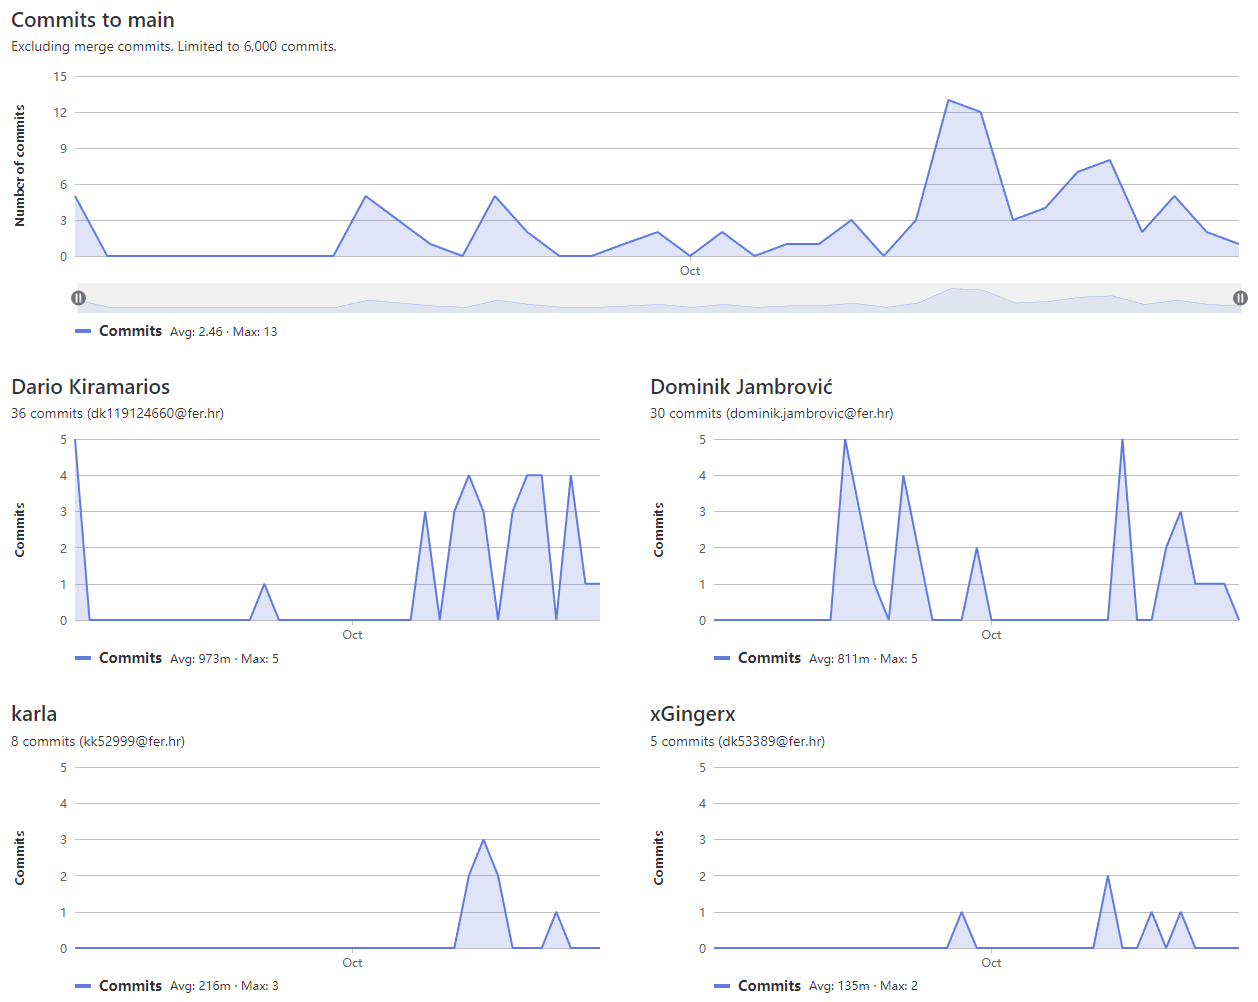
\includegraphics[width=1.1\textwidth,height=0.6\textheight]{slike/aktivnost1.png}}%
			\centering
			\caption{Prikaz commitova, prvi dio}
			\label{fig:promjene1}
		\end{figure}

        \begin{figure}[H]
			\makebox[\textwidth][c]{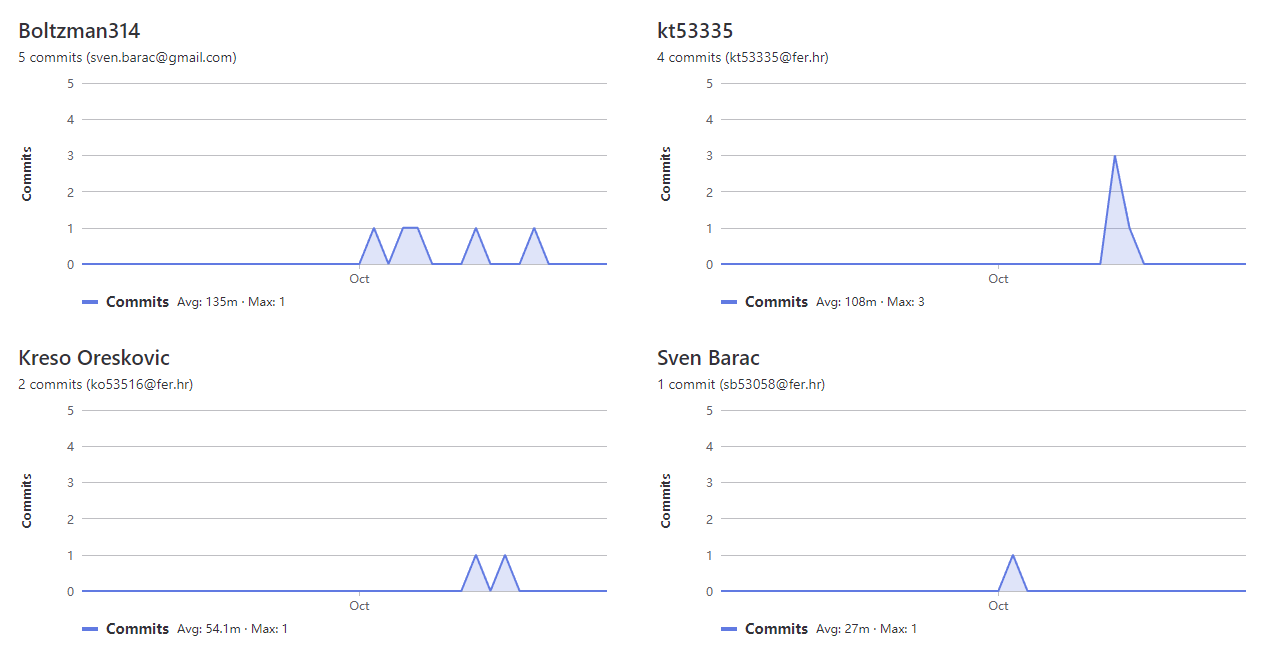
\includegraphics[width=1.1\textwidth,height=0.45\textheight]{slike/aktivnost2.png}}%
			\centering
			\caption{Prikaz commitova, drugi dio}
			\label{fig:promjene2}
		\end{figure}